\documentclass{standalone}
\usepackage{tikz}
\begin{document}
    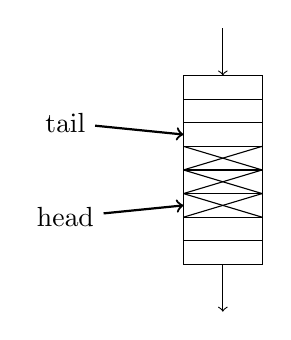
\begin{tikzpicture}[yscale=.6]
        \draw (-.5,-2) rectangle (.5,2);
        \foreach \i in {-1.5, -1, ..., 1.5}{
            \draw (-.5,\i) -- (.5,\i);
        }
        \draw [->] (0,3) -- (0,2);
        \draw [->] (0,-2) -- (0,-3);
        \node (b) at (-2,-1) {head};
        \node (e) at (-2,1) {tail};
        \draw [thick,->] (b) -- (-.5,-.75);
        \draw [thick,->] (e) -- (-.5,.75);
        \foreach \i in {-1,-.5,0}{
            \draw (-.5,\i) -- (.5,\i+.5);
            \draw (.5,\i) -- (-.5,\i+.5);
        }
    \end{tikzpicture}
    \end{document}
